%%&program=xelatex
%&encoding=UTF-8 Unicode
% SVN keywords
% $Author$
% $Date$
% $Revision$
% $URL$
\documentclass[a4paper,12pt]{article}      
%
\usepackage{ifxetex}% for XELATEX, or PDFlatex
\usepackage{ifplatform} 
%
\ifxetex
	\usepackage{polyglossia} \setmainlanguage{portuges}
	\usepackage{fontspec}
	\ifwindows
		\setmainfont[Ligatures=TeX]{Garamond}
		\setsansfont[Ligatures=TeX]{Gill Sans MT}
		\setmonofont{Consolas}
%		\setmonofont[Scale=MatchLowercase]{Courier}
	\fi
	\iflinux
		\setmainfont[Ligatures=TeX]{Linux Libertine O}
		\setsansfont[Ligatures=TeX,Scale=MatchLowercase]{Linux Biolinum}
		\setmonofont[Scale=MatchLowercase]{Courier}
	\fi
	\ifmacosx
	% add settings
	% Use xelatex -no-shell ...
	% Use xelatex -no-shell ...
		\setmainfont[Ligatures=TeX]{Garamond}
		\setsansfont[Ligatures=TeX]{Helvetica}
		\setmonofont{Consolas}
	\fi
	\usepackage{xcolor,graphicx} 
\else
	\usepackage[portuguese]{babel}
	%\usepackage[latin1]{inputenc}
	\usepackage[utf8]{inputenc}
	\usepackage[T1]{fontenc}
	\usepackage{graphics}                 % Packages to allow inclusion of graphics
	\usepackage{color}                    % For creating coloured text and background
\fi

%\usepackage{hyperref}                 % For creating hyperlinks in cross references
\usepackage{enumitem}
\setlist{nolistsep}


\usepackage{amsmath,amssymb,amsfonts} % Typical maths resource packages
\usepackage[retainorgcmds]{IEEEtrantools}
\usepackage{caption}

\oddsidemargin 0cm
\evensidemargin 0cm

\pagestyle{myheadings}         % Option to put page headers
                               % Needed \documentclass[a4paper,twoside]{article}
\markboth{{\small \it  Laboratório de Física Experimental Básica}}
{{\small\it MEFT - 1º Sem.  2015/2016} }

\addtolength{\hoffset}{-0.5cm}
\addtolength{\textwidth}{2.5cm}
\addtolength{\topmargin}{-1.5cm}
\addtolength{\textheight}{3cm}

%\textwidth 15.5cm
%\topmargin -1.5cm
\setlength{\parindent}{0pt}
\setlength{\parskip}{1ex  plus  0.5ex  minus  0.2ex}
%\parindent 0.5cm
%\textheight 25cm
%\parskip 1mm


% Math macros
\newcommand{\ud}{\,\mathrm{d}} 
\newcommand{\HRule}{\rule{\linewidth}{0.5mm}}

\author{Prof. Bernardo B. Carvalho} 

%%%%, Bernardo Brotas Carvalho\\bernardo@ipfn.ist.utl.pt} 
\date{ Outubro 2012} 

\begin{document} 

	
\includegraphics[width=0.2\textwidth]{../logo-ist}%\\[1cm]  %%  Logo_IST_color

	\HRule \\[0.5cm]
	{ \huge \sf  \textsc{A Propagação de Ondas Mecânicas em Meios Sólidos Homogéneos.}} \\[0.4cm] % \bfseries 
	{ \large \bfseries Propriedades Elásticas e as Constantes de Elasticidade}\\
	\HRule \\%[0.5cm]

\section{\sf Resumo do fundamento teórico do método utilizado}
Quando as forças exteriores aplicadas a um corpo sólido provocam pequenas deformações que lhes são proporcionais (lei de Hooke), e se as deformações cessarem quando as forças deixarem de actuar, o comportamento desses materias é bem descrito pela Teoria da Elasticidade. Pode mostrar-se que as diferentes propriedades físicas são obtidas em função das constantes elásticas do material.

\subsection{\sf Forças normais }

Para uma barra prismática de comprimento $l$ e secção $A$ (altura $h$ e largura $w$) actuada por forças de intensidade $F$, normais às bases e uniformes em toda a secção, por exemplo de tracção, vai observar-se um alongamento (“\emph{stretching}”) $\Delta l$ proporcional ao esforço, como ilustrado esquematicamente na figura 1. Se o esforço fosse de compressão o alongamento seria $\Delta l<0$. 


\begin{minipage}[c]{0.6\textwidth}
%\begin{figure}[!htb]  
\begin{center}
%trim=l b r t
%	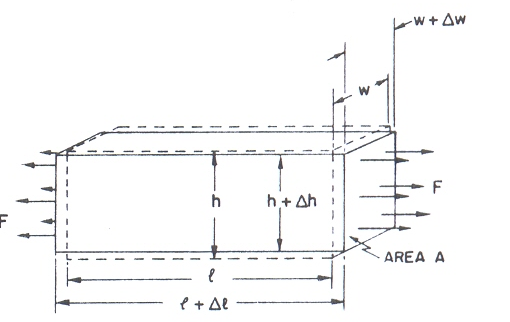
\includegraphics[trim=3mm 3mm 3mm 3mm, clip=true, width=0.8\linewidth]{moduloYoung}
	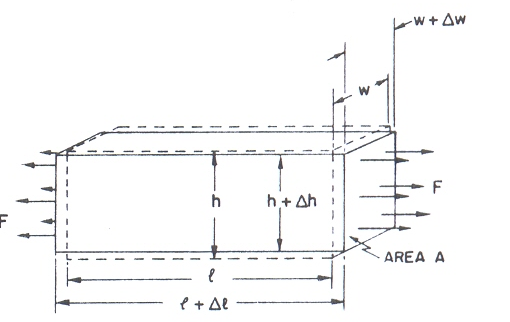
\includegraphics[width=0.8\linewidth]{moduloYoung}
\captionof{figure}{}
\label{fig:fig1}            
%	\caption{Montagem para determinar a Velocidade da Luz. \label{fig:Montagem}} 
\end{center}
%\end{figure}
\end{minipage}
\begin{minipage}[c]{0.4\textwidth}
\begin{equation}
	\label{eq:vc}
	 \frac{F}{A}  = Y  \frac{\Delta l}{l} 
\end{equation}
$Y$ é uma constante de elasticidade, \emph{módulo de Young} ou de \emph{compressão} (também representado por $E$) e que tem as dimensões de uma pressão (unidades Pascal no SI).
\end{minipage}

Alguns valores típicos para o módulo de Young são dados na tabela em baixo.

\begin{center}
\begin{tabular}{|r|l|}
\hline
\textbf{Material} & \textbf{Y (GPa)}\\
\hline
Borracha & 0.01 - 0.1\\
Nylon & 2 - 4 \\ % \cline{2-2}
Granito & 45 \\
Vidro & 50-90 \\
%\hline \hline
Latão & 50-90 \\
Aço  & 200 \\
Diamante  & 1220 \\
\hline
\end{tabular}
\end{center}

Como consequência da peça alongar e não estar submetida a restrições laterais, nas direções transversais vai observar-se um encurtamento $\Delta h$ e $\Delta w$ que é proporcional a $\Delta l$ mas de sinal contrário, tal que:

\begin{equation}
	\label{eq:poisson}
	 \frac{\Delta w}{w}  =   \frac{\Delta h}{h}  = - \sigma  \frac{\Delta l}{l} 
\end{equation}
em que $\sigma$ (também representado por $\nu$) é outra constante elástica, o \emph{coeficiente de Poisson}, adimensional e que varia no intervalo\footnote{Existe uma classe de materiais ou estruturas chamada auxéticos, em que o coeficiente de Poisson é negativo.} $[ 0,\;1/2 ] $.
Estas duas constantes elásticas caracterizam todas as propriedades elásticas dos materiais isótropos.

\begin{center}

\begin{tabular}{|r|c|}
\hline
\textbf{Material} & \textbf{$\sigma$}\\
\hline
Cortiça  & $\sim 0.0$ \\
%Nylon & 2 - 4 \\ 
Vidro & 0.18–0.3 \\
Betão & 0.2\\
%Latão & 50-90 \\
Aço  & .3 \\
Borracha & $\sim 0.5$\\
\hline
\end{tabular}
\end{center}


No caso da barra estar submetida a uma pressão idêntica, normal a todas as faces (é o caso de um corpo imerso num fluido submetido à pressão hidrostática) verifica-se uma diminuição de volume que faz intervir uma outra constante de elasticidade, volúmica, $K$ (módulo volúmico de compressão, \emph{“bulk modulus”}). Esta constante pode ser calculada da seguinte forma

\begin{equation}
	\label{eq:bulk}
	 \frac{F}{A}  =  -K \frac{\Delta V}{V} 
\end{equation}
Tem as dimensões de uma pressão, não é independente de $Y$ e $\sigma$ e pode provar-se que 

\begin{equation}
	\label{eq:K}
	 K=\frac{Y}{3\,(1-2\sigma)} 
\end{equation}
As forças de compressão ou tracção produzem variações de volume sem rotação das partículas do material.

Um meio é considerado anisótropo se as suas propriedades físicas dependem em cada ponto da direção considerada (é o caso dos meios cristalinos). Também os meios amorfos -- como os vidros, os plásticos, etc. -- quando são submetidos a esforços adquirem propriedades anisotrópicas\footnote{O carácter anisotrópicpo do material pode ser posto em evidência de forma visível colocando-o entre dois polaróides cruzados. 
Se o material é isotrópico, a interposição no par de polaróides não altera a fraca intensidade luminosa, qualquer que seja a sua orientação. Em contraste, quando o material entre polaróides é anisotrópico, observam-se padrões de cores, que mudam com a orientação e com as tensões aplicadas.}.

No caso de um meio anisotrópico os alongamentos para o mesmo esforço mecânico dependem das direções, e os diferentes coeficientes de proporcionalidade, i.e., os módulos de elasticidade são elementos do \emph{tensor de elasticidade}. A caraterização destes materiais exige o conhecimento de um grande número de elementos do tensor ($81=3^4$, que se reduzem a 21 valores independentes).

\subsection{\sf Forças tangenciais }
\begin{center}
	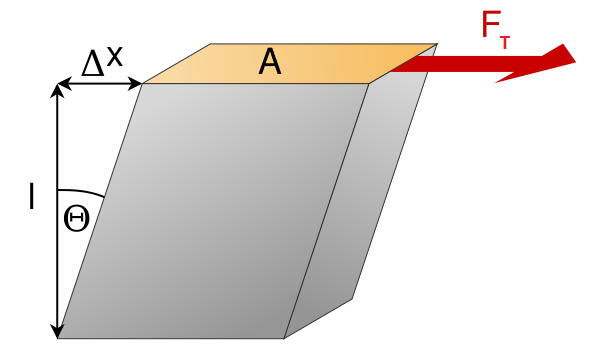
\includegraphics[width=0.45\linewidth]{602px-Shear_scherung}
	\captionof{figure}{\label{fig:fig2}}
\end{center}
Uma barra parelepipédica fixa pela base inferior, se for submetida a um esforço tangencial, como exemplificado na figura \ref{fig:fig2}, deforma-se de modo que as diferentes camadas deslizam umas sobre as outras, não variando o volume. Esse deslize das diferentes camadas pode ser caraterizado pelo ângulo 
$\theta$ que depende da força $F_T$ e da rigidez do material:

\begin{equation}
	\label{eq:shear}
	 \frac{F_T}{A} = \mu \, \theta 
\end{equation}

O coeficiente $\mu$ (também representado por $G$) é o módulo de rigidez (“cisalhamento” ou \emph{“shear modulus”}). Pode provar-se que 
\begin{equation}
	\label{eq:mu}
	 \mu  = \frac{Y}{2(1 +\sigma )}
\end{equation}
Quando as forças tangenciais aplicadas a uma barra cilíndrica, de comprimento $L$ e raio $r$, fixada pela base (situada à esquerda) constituem um binário, por exemplo como o da figura 3, a peça vai torcer.

\begin{center}
	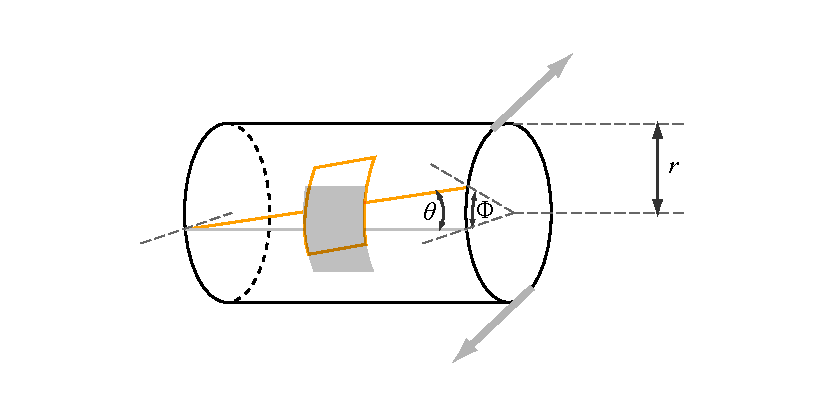
\includegraphics[width=0.7\linewidth]{rotac2}
	\captionof{figure}{\label{fig:fig3}}
\end{center}

Qualquer das geratrizes roda de um ângulo $\theta$ (que satisfaz a equação 	\ref{eq:shear}) e que define na base, onde o binário de forças atua, um ângulo $\Phi$. Esse ângulo depende do momento do binário e da rigidez da peça segundo 
\begin{equation}
	\label{eq:binario}
	 N= \mu \frac{\pi\,r^4}{2\,L} \Phi 
\end{equation}

\subsection{\sf Velocidades de propagação  }

As velocidades das ondas mecânicas que se propagam nos meios sólidos que se comportam como meios elásticos só dependem das constantes de elasticidade e da massa volúmica $\rho$.
Assim, os esforços de compressão/tracção produzem ondas longitudinais\footnote{As ondas longitudinais e transversais são referidas, por analogia com as ondas sísmicas, como ondas P (Primárias) e S (Secundárias).} 
%\footnote{As ondas P em sismologia. As Ondas S, são transversais.} 
que se propagam com velocidade $v_L$, tendo como suporte o movimento harmónico longitudinal das partículas do meio. Para uma barra temos
\begin{equation}
	\label{eq:vL}
	 v_L = \sqrt{\frac{Y}{\rho}}
\end{equation}

No caso de um corpo i.e. uma peça “volúmica”, em que as distâncias transversais não sejam muito inferiores à distância longitudinal (o comprimento da peça) a expressão (\ref{eq:vL}) tem que ser corrigida de um fator multiplicativo $f$. De facto, o material circundante a cada hipotética barra restringe os movimentos transversais que foram observados na barra (ver equação \ref{eq:poisson}). Nesse caso o módulo de Young vem multiplicado pelo fator

\begin{equation}
	\label{eq:f}
	f = \frac{1-\sigma}{(1+\sigma)(1-2\sigma)} 
\end{equation}
de modo que na equação (\ref{eq:vc}) $Y$ é substituido por $Y'=f\,Y$.

Pode obter-se a expressão que substitui (\ref{eq:vL})  considerando um bloco que é sujeito a compressão/tracção mas em que não podem ocorrer contrações laterais. A expressão é a seguinte:
\begin{equation}
	\label{eq:vL2}
	 v_L = \sqrt{\frac{K + 4/3\,\mu}{\rho}}
\end{equation}
porque pode mostrar-se facilmente atendendo a (\ref{eq:K}) e (\ref{eq:mu}) que  $Y'=K + 4/3\mu$.

Os esforços tangenciais produzem ondas transversais que se propagam com velocidade $v_T$ graças aos movimentos harmónicos transversais das partículas ou rotações produzidas por um binário de forças. Estas ondas transversais podem vibrar numa determinada direção no plano transversal (fixa ou que segue uma lei de evolução) sendo a sua velocidade
% e são pois \emph{polarizáveis}, ao contrário das ondas longitudinais que não são polarizáveis.
\begin{equation}
	\label{eq:vT}
	 v_T = \sqrt{\frac{\mu}{\rho}}
\end{equation}
Para um corpo obtém-se
\begin{equation}
	\label{eq:v_L_T}
	\left(\frac{v_L}{v_T}\right)^2 =  \frac{2(1-\sigma)}{(1-2\sigma)} 
\end{equation}
expressão que permite, a partir da determinação experimental das velocidades $v_L$ e $v_T$, calcular o valor do coeficiente de Poisson $\sigma$. Verifica-se que $v_L$ é sempre superior a $v_T$  (a partir de (\ref{eq:v_L_T}) pode provar-se facilmente que $\sigma<1/2$).
A determinação experimental destas velocidades permite calcular os valores das constantes de elasticidade $K$ e $\mu$, desde que se conheça o valor da massa volúmica do material.

No caso de materiais anisotrópicos só um grande número de determinações permite calcular as constantes de elasticidade (componentes do tensor de elasticidade). Assim, para um paralelepípedo anisotrópico, quando se calculam as diferentes velocidades segundo as três direções, só é fácil calcular o \emph{coeficiente de anisotropia} $c.a.$ que se obtém pela seguinte expressão
\begin{equation}
	\label{eq:ca}
	c.a.= \frac{v_{max}-v_{min}}{v_{max}}
\end{equation}

%\subsubsection{\sf Questões a responder ANTES da sessão de Laboratório}

%\begin{enumerate}
%\item Descreva por palavras suas quais os objectivos do Trabalho que irá realizar na sessão de Laboratório (uma folha A4). Indique as expressões que irá utilizar para obter as grandezas experimentais, bem como as expressões para calcular as incertezas. Inclua esta parte também no Relatório. Este irá constituir o ÚNICO meio de consulta na Prova Individual.
%\item Para a experiência do Pêndulo e supondo que o fio de Nylon tem um diâmetro de $1\,mm $, calcule a partir da expressão (\ref{eq:vc}), qual a variação de comprimento 
%do fio entre a posição mais alta e mais baixa da trajetória. Qual a variação máxima que esta alteração do comprimento provoca no período?
%\item Explique a partir das relações (\ref{eq:mu})  e  (\ref{eq:v_L_T})  porque não podem existir ondas transversais em liquídos e gases. Como se pode utilizar esta propriedade 
%na exploração de campos de petróleo?
%\item Considere uma camada de água, com velocidade de propagação $V_L=1450 \,m/s$, sobre uma camada de rocha granítica (Considere $K_{gra}=50\,GPa$, $\mu_{gra}=24\,GPa$ e \\
%$\rho_{gra}=2700\,kg/m^3$). 
%Determine o angulo de incidência  das ondas P na interface da água para a rocha a partir no qual terá reflexão total.
%\end{enumerate}


\newpage
\section{\sf Protocolo Experimental}
Nesta experiência vão determinar-se as velocidades de propagação das ondas mecânicas a partir da medição de espaços e tempos em várias amostras cortadas em forma de prisma quadrangular reto, podendo as medidas ser realizadas segundo duas direções ortogonais.
 Calculam-se em seguida as constantes elásticas ($K$, $\mu$ e $\sigma$) para os materiais isotrópicos e o coeficiente de anisotropia $c.a.$ para os materiais anisotrópicos.
 
Dispõe-se de um gerador/recetor que emite impulsos elétricos, que são transformados em impulsos mecânicos por um transdutor piezoelétrico, bem acoplado a uma das faces da amostra. Na face oposta coloca-se outro transdutor, que após receber o impulso mecânico o transforma num sinal elétrico e o envia ao gerador/recetor.

O tempo de percurso -- que é relativamente curto já que as velocidades de propagação nos meios sólidos são da ordem do quilómetro por segundo -- é determinado com a ajuda dum osciloscópio, onde se observam o impulso emitido e o recebido depois de ter sido transmitido através da amostra numa determinada direção. 

\subsection{\sf Material utilizado}
\begin{itemize}
\item Gerador / receptor de sinais eléctricos, Sensores
\item Osciloscópio,
\item Cilindros metálicos para calibração (latão) e amostras de rochas e de ‘plexiglass’
\end{itemize}

\begin{center}
	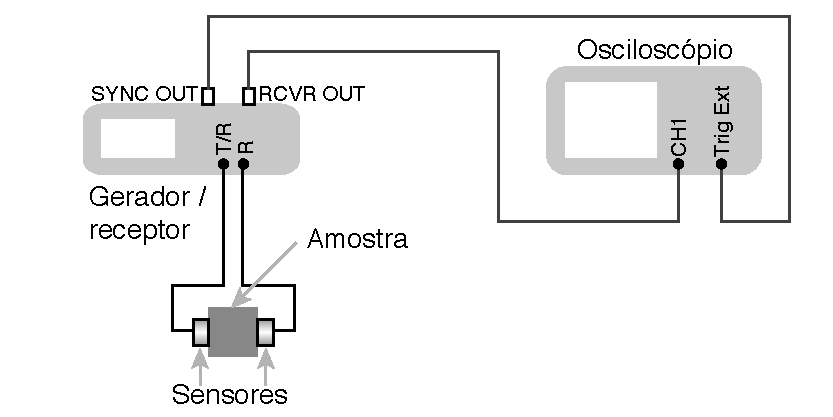
\includegraphics[width=0.7\linewidth]{esquema}
	\captionof{figure}{Esquema da montagem experimental. \label{fig:fig3}}
\end{center}


\begin{table}[htp]
\caption{Parâmetros do gerador / receptor.}
\begin{center}
\begin{tabular}{|r|c|}
\hline
\bf{Mode} & THRU (Through Transmission)\\
\hline
\bf{PRF (Pulse Repetition Freq.)} & 10.0 KHz\\
\hline
\bf{Energy} & 50 ou 100 $\mu$J\\
\hline
\bf{Damping} & 50 $\Omega$\\
\hline
\bf{HP Filt ( High Pass Filter)} & 300 KHz\\
\hline
\bf{LP Filt (Low Pass Filter)} & 5 MHz\\
\hline
\bf{Input Atten} & 50 dB\\
\hline
\bf{Output Atten} & 11.1 dB\\
\hline
\bf{Gain} & 40.0 dB\\
\hline
\bf{Sensitivity} & 24.8 dB\\
\hline
\end{tabular}
\end{center}
\end{table}


Verifique que o gerador/ receptor tem as funções definidas com as opções da tabela. Estabeleça as ligações como se indica no esquema [quando os sinais observados no osciloscópio forem muito fracos transfira o cabo ligado ao terminal Rcvr out para o terminal R do gerador]. Observe na base de tempo adequada o sinal emitido pelo gerador.

\subsection{\sf Calibração dos sensores}
Utilize os diferentes cilindros de latão e um par de sensores P (referência V 103 ). Para um melhor contacto sensor/cilindro, espalhe uma gota de líquido acoplante\footnote{Utilize óleo de silicone para as ondas longitudinais e o líquido viscoso para as ondas transversais.} na face de cada sensor que vai aplicar a cada extremidade do cilindro.

Observe no osciloscópio, no mesmo canal, o sinal emitido e o sinal recebido depois de ter atravessado o cilindro e determine o atraso entre os dois sinais. Repita para os outros cilindros. Estime o erro das observações.
Repita para todos os cilindros, usando agora os sensores S (referência V 153), tendo o cuidado de alinhar a marca (de polarização) existente no casquilho de cada sensor. Observe o que acontece ao sinal à medida que roda um dos sensores em relação ao outro.
Estime, usando um processo gráfico, a velocidade de propagação dos dois tipos de ondas, assim como o atraso temporal introduzido pela camada protectora de cada sensor (P e S).

\subsection{\sf Determinação da velocidade de propagação nas amostras}
Faça agora determinações semelhantes às anteriores para duas amostras de rochas e uma amostra de plexiglass com os sensores P. Repita a experiência para os dois pares de sensores S e observe o efeito da rotação, separadamente para cada um dos sensores.

Estime as velocidades de propagação das ondas P e S (e a correspondente precisão) segundo as direcções ensaiadas e conclua sobre a isotropia observada para esta propriedade. Analise as diferentes contribuições para as incertezas obtidas.

Para as amostras praticamente isótropas estime os módulos de elasticidade K, $\mu$ e $\sigma$ (e a correspondente precisão) e o coeficiente de anisotropia c.a. para as amostras anisótropas.



%\subsection{\sf Material utilizado}
%Conjuntos de sondas Transdutor/Recetor para ondas i) longitudinais e ii) tranversais. Aparelho emissor/recetor de impulsos. Conjunto de cilindros de latão para calibração de sondas. Osciloscópio.
%Paquímetro e Balança de pratos

%\subsection{\sf Procedimento Experimental}

%As ondas longitudinais e transversais observadas nas amostras são referidas, por analogia com as ondas sísmicas, como ondas P (principais) e S (secundárias).
%\begin{enumerate}
%\item Estabeleça as ligações necessárias para efetuar as medições de tempo de propagação nas amostras sólidas. Verifique se as regulações do aparelho de medida são as indicadas na folha de laboratório. Indetifique os dois conjuntos de transdutor (longitudinal/transversal) e para o segundo caso identifique a direção de polarização.
%\item Começe pelas medidas de calibração dos atrasos no conjunto de amostras de Latão, para as ondas P e S. Represente graficamente os  dados obtidos em função da distância percorrida. Verifique a linearidade e o atraso inicial (que é um erro sistemático).
%\item Para uma amostra isotrópica obtenha as velocidades de propagação(\ref{eq:vL2})  e  (\ref{eq:vT}) nas duas direções perpendiculares à altura dos blocos. 
%\item Calcule as constantes elásticas do material ($K$, $\mu$ e $\sigma$) e as respetivas incertezas.
%\item Se as velocidades de propagação diferirem de um valor superior ao intervalo de incerteza, calcule o coeficiente de anisotropia.
%\end{enumerate} 

\newpage
\section*{\sf Apêndice}
\subsection{\sf A equação de propagação por ondas (ondas planas)} 

Na aula teórica foi apresentada a forma de um campo vetorial $\vec{V}$ organizado em onda plana 
\begin{equation}
	\label{eq:onda}
	\vec{V}(x,t)=\vec{V}_{max} \sin \left(\frac{2\,\pi}{T}t - \frac{2\,\pi}{\lambda}x + \delta \right)
\end{equation}

A fase da onda $\phi = \frac{2\,\pi}{T}\,t - \frac{2\pi}{\lambda}\,x + \delta$  é o argumento da função trigonométrica e contém os parâmetros que caraterizam a periodicidade da onda $T$ e $\lambda$, bem como a desfasagem $\delta$ que dá conta do valor da amplitude no início do tempo e do espaço. Para simplificar, vamos considerar $\delta=0$ e só a intensidade do campo.

A velocidade de fase $v$ é definida como a velocidade a que se desloca um ponto de fase constante, i.e.  $v=(\frac{\ud x}{\ud t})_{\ud \phi=0}$. A condição $\ud \phi = 0$ equivale a $\frac{2\,\pi}{T}\,\ud t = \frac{2\,\pi}{\lambda}\,\ud x$, obtendo-se

\begin{equation}
	\label{eq:v}
	v=\frac{\lambda}{T} 
\end{equation}

Calculando $\frac{\partial V }{\partial x}, \;\frac{\partial V }{\partial t}, \;\frac{\partial^2 V }{\partial x^2}, \; \textrm{ e } \;\frac{\partial^2 V }{\partial t^2} $   e    obtém-se\footnote{Para simplificação da escrita usa-se $V$ em vez de $\vec{V}$. }

\begin{IEEEeqnarray}{lCr}
\frac{\partial V }{\partial x} = V_{max} \, (-\frac{2\,\pi}{\lambda}) \cos \phi &\qquad& \frac{\partial V }{\partial t} = V_{max} \, (+\frac{2\,\pi}{T}) \cos \phi\\
%
\frac{\partial^2 V }{\partial x^2} = -V_{max} \, \left(-\frac{2\,\pi}{\lambda}\right)^2 \sin \phi &\qquad& \frac{\partial^2 V }{\partial t^2} = -V_{max} \, \left(+\frac{2\,\pi}{T}\right)^2 \sin \phi
\end{IEEEeqnarray}

A partir das duas últimas expressões podemos escrever

\begin{equation}
	\label{eq:ondap}
-V_{max} (2 \pi)^2  \sin \phi = \lambda^2 \frac{\partial^2 V }{\partial x^2} = T^2 \, \frac{\partial^2 V }{\partial t^2} \Rightarrow 
\frac{\partial^2 V }{\partial x^2} = \frac{1}{v^2}  \, \frac{\partial^2 V }{\partial t^2}
\end{equation}

Esta última equação é a equação diferencial caraterística das ondas planas, que põe em evidência a velocidade de propagação de fase $v$. Qualquer campo escalar ou vetorial organizado em onda plana satisfaz a uma equação deste tipo.

\subsection{\sf A equação de propagação das ondas longitudinais nos sólidos} 

% http://www.acs.psu.edu/drussell/Demos/waves/wavemotion.html

Consideremos agora uma fatia elementar de uma barra cilíndrica de um material de massa volúmica $\rho$, de secção $A$ e espessura $\ud x$, submetida a duas forças de compressão normais à secção, numa face $F$ e na outra $F+\ud F$. Esta diferença $\ud F$ produz um deslocamento  $\ud \xi$  segundo o eixo do cilíndro.

A equação (\ref{eq:vc}) escreve-se agora em termos do deslocamento elementar da seguinte forma
\begin{equation}
	\label{eq:a4}
	 F = A \, Y \frac{\partial \xi }{\partial x} 
\end{equation}

A diferença $\ud F = \frac{\partial F }{\partial x} \ud x $ cria uma aceleração $a=\frac{\partial^2 \xi }{\partial t^2} $  sobre a massa elementar $\ud m= \rho\,A \ud x $ da fatia, tal que pela lei de Newton

\begin{equation}
	\label{eq:a5}
	 \ud F=\ud m\,a\Rightarrow \frac{\partial F }{\partial x} \ud x  =  \rho\,A \ud x \frac{\partial^2 \xi }{\partial t^2} \Rightarrow \frac{\partial F }{\partial x} = \rho\,A  \frac{\partial^2 \xi }{\partial t^2}
\end{equation}

Por outro lado, aplicando a derivada parcial em ordem a $x$ à equação (\ref{eq:a4}) obtém-se
\begin{equation}
	\label{eq:a6}
	\frac{\partial F }{\partial x} = A \, Y \frac{\partial^2 \xi }{\partial x^2}
\end{equation}	

Combinando (\ref{eq:a5}) e (\ref{eq:a6}) obtemos a equação :
\begin{equation}
	\label{eq:a7}
	\frac{\partial^2 \xi }{\partial x^2} - \frac{\rho}{Y} \frac{\partial^2 \xi }{\partial t^2} =0
\end{equation}	

Esta equação é caraterística duma onda plana que se propaga com velocidade de fase igual a $v=\sqrt{\frac{Y}{\rho}}$, a qual corresponde à velocidade longitudinal apresentada na equação (\ref{eq:vL}). 

\end{document} 